
\documentclass[a4paper,14pt]{extreport} % формат документа

%\documentclass[utf8x, 14pt]{G7-32}
\usepackage[warn]{mathtext}
\usepackage{amsmath}
\usepackage{cmap} % поиск в ПДФ
\usepackage[T2A]{fontenc} % кодировка
\usepackage[utf8]{inputenc} % кодировка исходного текста
\usepackage[english,russian]{babel} % локализация и переносы
\usepackage[left = 2cm, right = 1cm, top = 2cm, bottom = 2 cm]{geometry} % поля
\usepackage{listings}
\usepackage{graphicx} % для вставки рисунков
\usepackage{amsmath}
\usepackage{float}
\usepackage{longtable}
\usepackage{multirow}
\usepackage{pdfpages}
\graphicspath{{pictures/}}
\DeclareGraphicsExtensions{.pdf,.png,.jpg}
\newcommand{\anonsection}[1]{\section*{#1}\addcontentsline{toc}{section}{#1}}

\begin{document}
	
\begin{titlepage}
	
	\begin{table}[H]
		\centering
		\footnotesize
		\begin{tabular}{cc}
			\multirow{8}{*}{
\includegraphics[scale=0.35]{bmstu.jpg}}
			& \\
			& \\
			& \textbf{Министерство науки и высшего образования Российской Федерации} \\
			& \textbf{Федеральное государственное бюджетное образовательное учреждение} \\
			& \textbf{высшего образования} \\
			& \textbf{<<Московский государственный технический} \\
			& \textbf{университет имени Н.Э. Баумана>>} \\
			& \textbf{(МГТУ им. Н.Э. Баумана)} \\
		\end{tabular}
	\end{table}
	
	\vspace{-1.5cm}
	
	\begin{flushleft}
		\rule[-1cm]{\textwidth}{3pt}
		\rule{\textwidth}{1pt}
	\end{flushleft}
	
	\begin{flushleft}
		\small
		ФАКУЛЬТЕТ
		\underline{<<Информатика и системы управления>>\ \ \ \ \ \ \ 
			\ \ \ \ \ \ \ \ \ \ \ \ \ \ \ \ \ \ \ \ \ \ \ \ \ \ \ \ \ \ \ 
			\ \ \ \ \ \ \ \ \ \ \ \ \ \ \ } \\
		КАФЕДРА
		\underline{<<Программное обеспечение ЭВМ и
			информационные технологии>>
			\ \ \ \ \ \ \ \ \ \ \ \ \ \ \ \ \ \ \ \ }
	\end{flushleft}
	
	\vspace{2cm}
	
	\begin{center}
		\textbf{Лабораторная работа № 9} \\
		\textbf{Дисциплина:}  Компьютерные сети.  \\
		\textbf{Тема} 
		Изучение технологии виртуальных локальных \\ сетей (VLan) в сетевом симуляторе. Настройка маршрутизации между VLan.\\
		\textbf{Вариант №15} \\
	\end{center}

    \vspace{4cm}
    
	\begin{flushright}
		\begin{tabular}{rr}
			\textbf{Студент} & Неклепаева А.Н. \\
			\textbf{Группа} & ИУ7-73Б \\
			\textbf{Преподаватель} & Рогозин Н.О.   \\
		\end{tabular}
	\end{flushright}
	
	\vspace{7cm}
	
	\begin{center}
		Москва, 2020 г.
	\end{center}
	
\end{titlepage}

\textbf{Задача:} 

I. Назначить адреса подсетей:

a) Подсеть 1: 192.168.x.0 /24

b) Подсеть 2: 192.168.x+1.0 /24

c) Подсеть 3: 192.168.x+2.0 /24

II. Настроить поддержку трех виртуальных локальных сетей (VLan 10, 20, 30) на коммутаторе.

III. Настроить маршрутизацию между виртуальными локальными сетями на маршрутизаторе.

IV. Выделить и озаглавить на схеме каждую виртуальную локальную сеть.

\textbf{Результаты работы:}

I. Разделение на подсети.

На рис. \ref{fig:podseti} указаны диапазоны адресов для каждой подсети.

\begin{figure}[H]
	\centering
	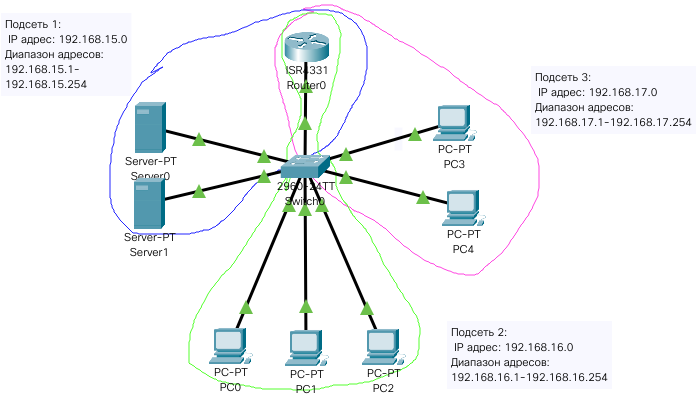
\includegraphics[width=1\linewidth]{podseti}
	\caption{}
	\label{fig:podseti}
\end{figure}

II. Настройка поддержки трех виртуальных локальных сетей (VLan 10, 20, 30) на коммутаторе.

В созданные виртуальные локальные сети необходимо добавить физические интерфейсы коммутатора. Для этого используется команда 

interface range range\underline{ }begin-range\underline{ }end,

где range\underline{ }begin - начало диапазона, 

range\underline{ }end - конец диапазона.

switchport mode access - переводит физический интерфейс в access режим.

switchport access vlan vlan\underline{ }num - указывает, для какой вирт. локальной сети передает данные физический интерфейс.

switchport mode trunk - переводит физический интерфейс в trunk режим.

В CLI коммутатора вводились следующие команды рис. \ref{fig:2}:

\begin{figure}[H]
	\centering
	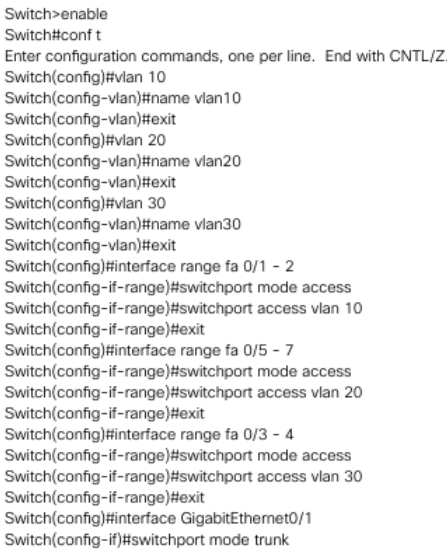
\includegraphics[width=0.7\linewidth]{2}
	\caption{}
	\label{fig:2}
\end{figure}

В VLAN Database были добавлены следующие записи рис. \ref{fig:21}:

\begin{figure}[H]
	\centering
	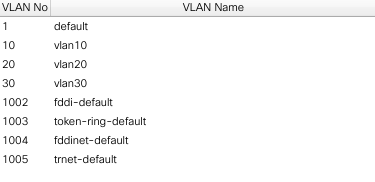
\includegraphics[width=0.7\linewidth]{2_1}
	\caption{}
	\label{fig:21}
\end{figure}

III. Настройка маршрутизации между виртуальными локальными сетями на маршрутизаторе.

Команда перехода в режим настройки подинтерфейса выполняется из режима глобальной конфигурации; используется для создания нового, если подинтерфейса с таким именем не существует:

interface interface\underline{ }name.subinterface\underline{ }name,

например

int g0/0/0.1

Для каждого подинтерфейса необходимо выполнить команду, которая позволит инкапсулировать передаваемые данные по стандарту IEEE 802.1Q:

encapsulation dot1q vlan\underline{ }num - 

где vlan\underline{ }num - номер VLan данные от которой будет получать

 указанный интерфейс

В CLI маршрутизатора вводились следующие команды рис. \ref{fig:3}:

\begin{figure}[H]
	\centering
	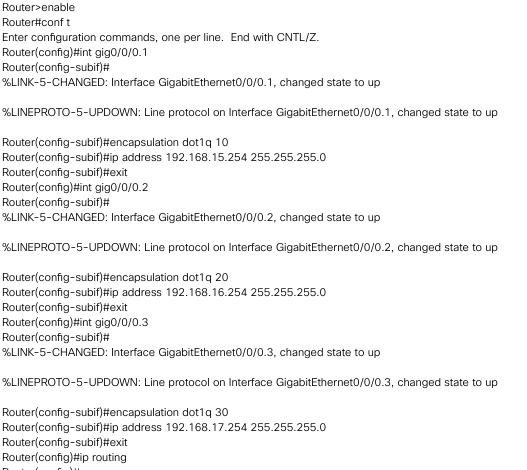
\includegraphics[width=1\linewidth]{3}
	\caption{}
	\label{fig:3}
\end{figure}

В качестве шлюза по умолчанию в конечных узлах во всех трех подсетях были выставлены адреса, приведенные выше.

IV. Выделение на схеме каждой виртуальной локальной сети.

Выделение каждой виртуальной локальной сети показано на рис. \ref{fig:4}:

\begin{figure}[H]
	\centering
	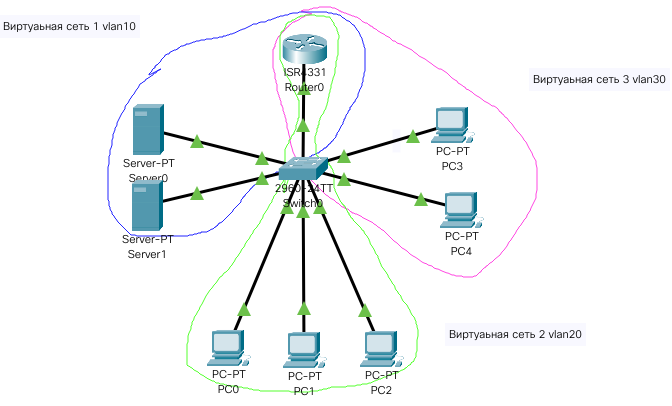
\includegraphics[width=1\linewidth]{4}
	\caption{}
	\label{fig:4}
\end{figure}

Пинг компьютером PC0 компьютера PC3 показан на рис. \ref{fig:5}:

\begin{figure}[H]
	\centering
	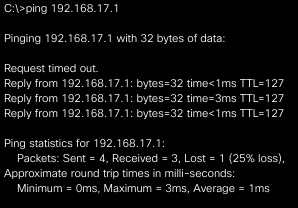
\includegraphics[width=0.7\linewidth]{5}
	\caption{}
	\label{fig:5}
\end{figure}

\end{document}
	